\documentclass[tcc1]{uftex}

\usepackage[alf,abnt-emphasize=bf]{abntex2cite}
\usepackage{amsmath}
\usepackage{booktabs}
\usepackage{float}
\usepackage{url}

\begin{document}

\title{Reescrita e Implementacao de um Algoritmo de Divisao e Conquista para Segmentacao em Microscopia Eletronica}
\author{Vinicius Wanderley}{Arruda}
\advisor{Prof.}{Warley}{Gramacho}{}
\department{CC}
\class{Projeto e Analise de Algoritmos}
\date{09}{06}{2026}

\keyword{Divisao e conquista}
\keyword{Segmentacao de imagens}
\keyword{Cryo-EM}
\keyword{Watershed}
\keyword{Analise de algoritmos}

\foreignkeyword{Divide and conquer}
\foreignkeyword{Image segmentation}
\foreignkeyword{Cryo-EM}
\foreignkeyword{Watershed}
\foreignkeyword{Algorithm analysis}

\maketitle
\frontmatter

\begin{abstract}
Este trabalho reescreve e discute o artigo ``A Divide and Conquer Algorithm for Electron Microscopy Segmentation'', de Jebril et al. O problema abordado e a segmentacao de mapas de densidade produzidos por microscopia crioeletronica, etapa importante para separar cadeias ou subunidades de uma macromolecula. O artigo combina uma segmentacao preliminar baseada em watershed com uma estrategia de divisao e conquista. Na versao proposta, o mapa de densidade e dividido recursivamente em subimagens menores, cada subproblema e segmentado localmente e, ao final, as regioes parciais sao combinadas por uma fase de merge ate atingir o numero esperado de regioes. Como parte pratica, foi desenvolvida uma implementacao didatica em Python, usando matrizes 2D sinteticas para demonstrar as etapas de divisao, resolucao dos subproblemas e combinacao. A implementacao nao substitui ferramentas especializadas de cryo-EM, mas reproduz a estrutura algoritmica central do artigo e permite observar a aplicacao da tecnica de divisao e conquista.
\end{abstract}

\begin{foreignabstract}
This work rewrites and discusses the article ``A Divide and Conquer Algorithm for Electron Microscopy Segmentation'', by Jebril et al. The addressed problem is the segmentation of density maps produced by cryo-electron microscopy, an important step for separating molecular chains or subunits. The article combines a preliminary watershed-based segmentation with a divide-and-conquer strategy. In the proposed method, the density map is recursively divided into smaller subimages, each subproblem is segmented locally, and the partial regions are later merged until the expected number of final regions is reached. As the practical part of this assignment, a didactic Python implementation was developed using synthetic 2D matrices to demonstrate division, subproblem solving, and combination. Although simplified when compared with real cryo-EM tools, the implementation reproduces the main algorithmic structure of the original method.
\end{foreignabstract}

\tableofcontents

\mainmatter

\chapter{Introducao}

A microscopia crioeletronica, conhecida como cryo-EM, permite gerar mapas tridimensionais de densidade para moleculas biologicas. Esses mapas sao usados para estudar a estrutura de proteinas e complexos macromoleculares, especialmente quando metodos tradicionais, como cristalografia por raios X e ressonancia magnetica nuclear, sao mais dificeis de aplicar. Uma etapa importante nesse fluxo e segmentar o mapa em regioes associadas as cadeias ou subunidades da molecula.

O artigo escolhido para esta atividade, de \citeonline{jebril2020divide}, propoe um algoritmo de segmentacao baseado em divisao e conquista. A ideia central e evitar que a etapa de combinacao de regioes seja executada de forma muito cara sobre o mapa inteiro. Para isso, o mapa e dividido em partes menores; cada parte e segmentada separadamente; e as regioes obtidas nos subproblemas sao mescladas ate formar a segmentacao final.

A escolha deste artigo se encaixa no objetivo da atividade porque a tecnica de divisao e conquista nao aparece apenas como inspiracao geral. Ela compoe diretamente o metodo: ha uma etapa de divisao do mapa, uma chamada recursiva para resolver subproblemas e uma etapa de conquista, na qual as regioes parciais sao combinadas.

\chapter{Conceitos Necessarios}

Antes de descrever o algoritmo, e importante apresentar alguns conceitos usados no artigo. Como o trabalho esta ligado a uma aplicacao de bioinformatica e processamento de imagens, alguns termos podem nao ser familiares em uma primeira leitura.

\section{Microscopia Crioeletronica}

A microscopia crioeletronica, ou \textit{cryo-electron microscopy} (cryo-EM), e uma tecnica experimental usada para observar moleculas biologicas em escala muito pequena. Na cryo-EM, a amostra e rapidamente congelada, preservando sua estrutura em um estado proximo ao natural. Em seguida, um microscopio eletronico captura imagens da amostra. A partir dessas imagens, ferramentas computacionais constroem um mapa tridimensional que representa a forma aproximada da molecula.

Essa tecnica e muito util para estudar proteinas e grandes complexos moleculares. Ela se tornou importante porque algumas moleculas sao dificeis de analisar por metodos tradicionais, como cristalografia por raios X. No contexto do artigo, a cryo-EM fornece o dado de entrada que precisa ser segmentado.

\section{Mapa de Densidade e Voxel}

O resultado computacional usado no artigo e chamado de mapa de densidade. Esse mapa pode ser entendido como uma imagem tridimensional em que cada ponto guarda um valor numerico de intensidade. Valores maiores indicam regioes em que ha maior probabilidade de existir materia biologica, como atomos ou partes de uma proteina.

Em uma imagem 2D, o menor elemento e chamado de pixel. Em uma imagem 3D, o equivalente e chamado de voxel, abreviacao de \textit{volumetric pixel}. Assim, um voxel e uma pequena celula de volume dentro do mapa tridimensional. Este e o termo usado no artigo para representar cada unidade do mapa de densidade. Quando o algoritmo fala em agrupar voxels, ele esta falando em juntar pequenas partes do volume para formar regioes maiores, associadas a cadeias ou subunidades da molecula.

\section{Segmentacao}

Segmentar uma imagem significa dividi-la em regioes com significado. No caso de cryo-EM, a segmentacao busca separar o mapa de densidade em partes que correspondam as subunidades da molecula. Por exemplo, se uma proteina possui duas cadeias principais, uma boa segmentacao deve produzir regioes que se aproximem dessas duas cadeias.

Essa etapa facilita a modelagem posterior, pois permite que cada parte da molecula seja analisada separadamente. Se a segmentacao estiver errada, regioes diferentes podem ser misturadas ou uma mesma cadeia pode ser quebrada em partes demais.

\section{\textit{Watershed}}

O \textit{watershed} e uma tecnica classica de segmentacao. A ideia vem de uma analogia com relevo geografico. Imagine uma imagem como uma superficie: pontos de maior ou menor intensidade formam montanhas, vales e bacias. O algoritmo tenta separar regioes de acordo com esses relevos, como se a agua preenchesse diferentes bacias hidrográficas.

No artigo, o watershed e usado como base para criar regioes preliminares. Primeiro, pontos de baixa densidade sao descartados por meio de um limiar. Depois, os pontos restantes sao processados de acordo com sua densidade e associados a regioes vizinhas. Essa etapa pode gerar muitas regioes pequenas; por isso, o algoritmo precisa de uma fase posterior de combinacao.

\section{Limiar de Densidade}

O limiar de densidade e um valor minimo usado para decidir quais voxels serao considerados relevantes. Se a densidade de um voxel fica abaixo desse valor, ele e tratado como ruido ou fundo da imagem. Se fica acima, ele participa da segmentacao. Esse parametro e importante porque um limiar muito baixo pode incluir ruido, enquanto um limiar muito alto pode remover partes importantes da molecula.

\section{Segger, EMDB e PDB}

O Segger e uma ferramenta de segmentacao usada em mapas de cryo-EM. No artigo, ele aparece como base de comparacao, pois tambem utiliza estrategias relacionadas a watershed e agrupamento de regioes.

O EMDataBank (EMDB) e uma base publica de mapas de microscopia eletronica. Ja o Protein Data Bank (PDB) e uma base publica de estruturas moleculares. Os autores usam mapas do EMDB e modelos do PDB para comparar as regioes segmentadas pelo algoritmo com regioes de referencia.

\chapter{Problema e Artigo Base}

O problema tratado e a segmentacao de imagens volumetricas de cryo-EM. Em termos computacionais, a entrada pode ser representada como um mapa de densidade $D$, composto por voxels. Cada voxel possui uma intensidade ou densidade. A saida esperada e um conjunto de regioes que agrupam voxels pertencentes a uma mesma subunidade molecular.

Segundo o artigo, a segmentacao manual pode ser demorada e depende de conhecimento especializado. Ferramentas automaticas e semiautomaticas, como o Segger, usam watershed e agrupamento de regioes, mas ainda podem apresentar supersegmentacao ou exigir intervencao do usuario. A proposta dos autores e acelerar o processo por meio de uma estrategia de divisao e conquista sobre o mapa de densidade.

Nos experimentos originais, os autores utilizaram 10 mapas reais de cryo-EM obtidos do EMDataBank e modelos estruturais do Protein Data Bank para construir cortes de referencia \cite{emdb,berman2000pdb}. O metodo foi comparado com o Segger, ferramenta usada como referencia pratica para segmentacao de mapas de cryo-EM \cite{pintilie2010segger}.

\chapter{Descricao do Algoritmo}

O codigo-fonte desenvolvido para esta reescrita esta disponivel em repositorio publico no GitHub \cite{arruda2026paa}. A implementacao foi construida como uma versao didatica do algoritmo do artigo, preservando a estrategia de divisao, resolucao recursiva dos subproblemas e combinacao das regioes.

\section{Segmentacao Preliminar}

O algoritmo do artigo inicia com uma segmentacao preliminar baseada em watershed. Essa etapa possui duas fases.

Na primeira fase, o mapa de densidade e suavizado e filtrado por um limiar. Voxels com densidade abaixo do limiar sao removidos por serem considerados ruido ou regioes pouco relevantes. Em seguida, os voxels restantes sao processados em ordem decrescente de densidade. Se um voxel nao possui vizinhos ja associados a alguma regiao, ele inicia uma nova regiao. Caso contrario, ele e atribuido a regiao vizinha predominante.

Na segunda fase, as regioes preliminares sao mescladas. Cada regiao possui um maximo local, isto e, um voxel com maior densidade dentro da regiao. O algoritmo ordena esses maximos e procura, para regioes de menor densidade, o maximo local que representa sua subida mais ingreme. A regiao de origem e entao mesclada a regiao associada a esse maximo. Esse processo se repete ate que o numero de regioes seja menor ou igual a $K$, onde $K$ e o numero desejado de segmentos finais.

\section{Divisao}

Na versao por divisao e conquista, o mapa $D$ e dividido em aproximadamente $\sqrt{n}$ subimagens, cada uma com aproximadamente $\sqrt{n}$ voxels, sendo $n$ o numero total de voxels. Essa escolha difere da divisao binaria classica, pois busca reduzir o custo da etapa de merge sem criar apenas dois subproblemas grandes.

\section{Subproblemas}

Cada subimagem $D_i$ e segmentada recursivamente pelo mesmo algoritmo. Quando o subproblema se torna pequeno o suficiente, aplica-se a segmentacao preliminar. Assim, a base da recursao e um bloco pequeno, no qual o custo do watershed e da combinacao local e aceitavel.

\section{Combinacao}

A etapa de combinacao recebe as regioes produzidas pelas subimagens. Como cada subproblema pode gerar ate $K$ regioes, a combinacao trabalha com aproximadamente $K\sqrt{n}$ regioes intermediarias. A fase de merge da segmentacao preliminar e reaplicada sobre essas regioes para chegar a no maximo $K$ regioes finais.

Essa etapa e a ``conquista'' do algoritmo: as solucoes parciais sao reorganizadas e unificadas, produzindo uma segmentacao coerente para o mapa original.

\chapter{Analise de Complexidade}

No algoritmo preliminar, a primeira fase e dominada pela ordenacao dos voxels, com custo $O(n \log n)$. A segunda fase depende do numero $m$ de regioes preliminares e possui custo indicado no artigo como $O(m^2 \log m)$. Assim, a segmentacao preliminar e analisada como:

\begin{equation}
O(n \log n + m^2 \log m).
\end{equation}

O problema e que, para mapas grandes, mesmo que $m$ seja menor que $n$, o termo quadratico pode se tornar caro. A estrategia de divisao e conquista reduz esse gargalo. No artigo, a recorrencia da versao square-root divide-and-conquer e apresentada como:

\begin{equation}
T(n) = \sqrt{n}T(\sqrt{n}) + c(K\sqrt{n})^2\log(Kn),
\end{equation}

onde $K$ e o numero de regioes desejadas. Como $K$ e tratado como parametro pequeno em relacao ao tamanho do mapa, os autores simplificam a complexidade para:

\begin{equation}
O(K^2 n \log n) = O(n \log n).
\end{equation}

Portanto, a otimizacao principal do artigo esta em substituir uma combinacao global potencialmente cara por combinacoes menores e recursivas.

\chapter{Implementacao Desenvolvida}

A implementacao foi desenvolvida em Python e esta localizada na pasta \texttt{codigo/} do repositorio \cite{arruda2026paa}. Como os dados reais de cryo-EM sao volumetricos, grandes e dependem de formatos especificos, a versao implementada usa matrizes 2D sinteticas. Essa decisao torna a demonstracao mais simples, mas preserva as etapas fundamentais do algoritmo.

O programa implementa:

\begin{itemize}
  \item geracao de um mapa sintetico de densidade;
  \item filtragem por limiar;
  \item inicializacao de regioes em ordem decrescente de densidade;
  \item merge por maximos locais e subida mais ingreme;
  \item divisao recursiva em blocos;
  \item combinacao das regioes parciais;
  \item visualizacao do mapa original e das regioes finais.
\end{itemize}

\section{Trecho Principal}

O trecho abaixo resume a funcao de divisao e conquista implementada:

\begin{lstlisting}[language=Python,caption={Funcao principal da segmentacao por divisao e conquista.}]
def segmentacao_divisao_conquista(mapa, limiar, k_final, tamanho_base=32):
    n = mapa.size
    if n <= tamanho_base * tamanho_base:
        return segmentacao_preliminar(mapa, limiar, k_final)

    partes_por_eixo = max(2, round(n ** 0.25))
    labels_global = np.zeros_like(mapa, dtype=int)
    deslocamento = 0

    for l0, l1, c0, c1, bloco in dividir_em_blocos(mapa, partes_por_eixo):
        resultado_bloco = segmentacao_divisao_conquista(
            bloco, limiar, k_final, tamanho_base
        )
        labels_bloco = resultado_bloco.labels.copy()
        mascara = labels_bloco != BACKGROUND
        labels_bloco[mascara] += deslocamento
        labels_global[l0:l1, c0:c1] = labels_bloco
        deslocamento = int(labels_global.max())

    return mesclar_regioes(mapa, labels_global, k_final)
\end{lstlisting}

\section{Exemplo Pratico}

A Figura~\ref{fig:demo-segmentacao} mostra a execucao da implementacao em uma matriz sintetica. A esquerda esta o mapa de densidade gerado artificialmente. A direita aparecem as regioes finais depois da divisao, resolucao recursiva e combinacao.

\begin{figure}[H]
  \centering
  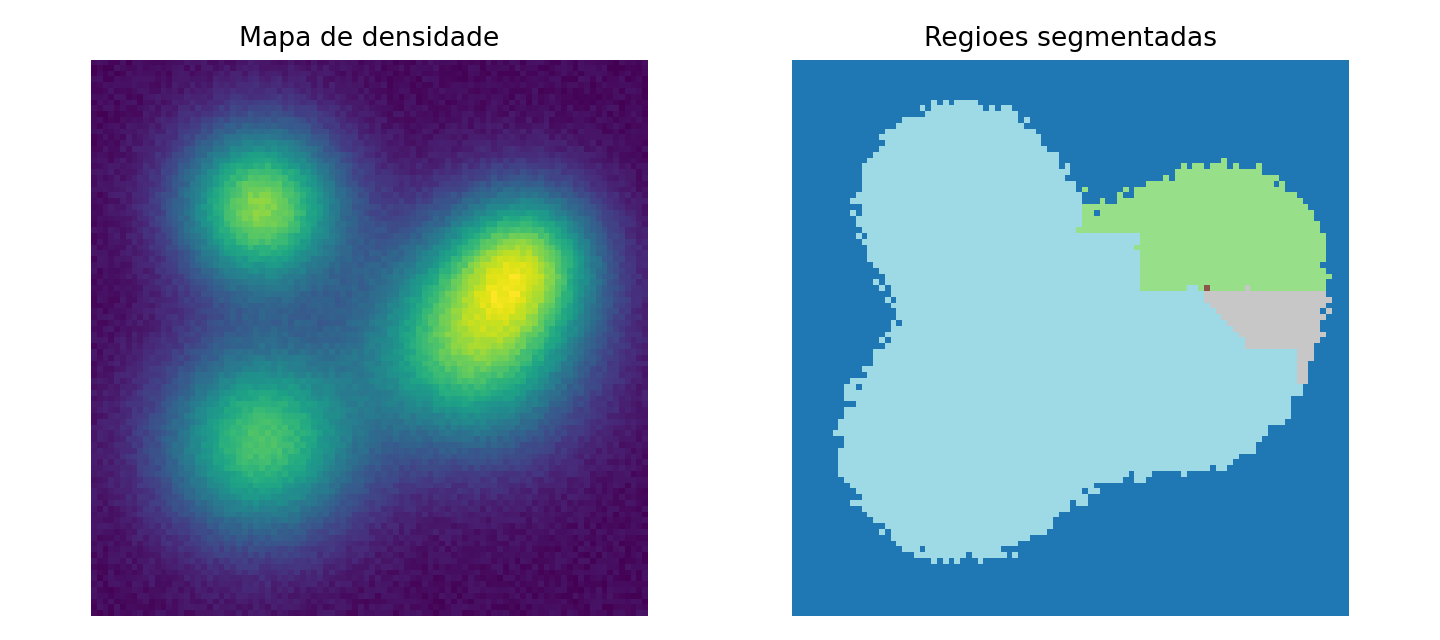
\includegraphics[width=0.85\textwidth]{figuras/demo_segmentacao.png}
  \caption{Demonstracao da segmentacao por divisao e conquista em matriz sintetica.}
  \label{fig:demo-segmentacao}
\end{figure}

Na execucao padrao, o algoritmo encontra 4 regioes, usando limiar de densidade $0{,}18$, tamanho base 32 e uma matriz $96 \times 96$.

\section{Como Executar}

Para executar a implementacao, basta instalar as dependencias e rodar o script principal:

\begin{lstlisting}[language=bash,caption={Comandos para executar a implementacao.}]
cd codigo
python -m pip install -r requirements.txt
python segmentacao_dc.py
\end{lstlisting}

O programa tambem aceita parametros opcionais, como tamanho da matriz, limiar de densidade, numero alvo de regioes, tamanho base da recursao, semente aleatoria e caminho da imagem de saida. Por exemplo:

\begin{lstlisting}[language=bash,caption={Execucao com parametros personalizados.}]
python segmentacao_dc.py --tamanho 128 --limiar 0.20 --regioes 4 --tamanho-base 32 --saida resultados/teste.png
\end{lstlisting}

\chapter{Comparacoes e Otimizacoes}

O artigo compara o metodo proposto com o Segger. Os autores destacam que uma comparacao perfeitamente justa e dificil, pois o Segger e uma ferramenta interativa, enquanto o metodo proposto recebe parametros como limiar e numero desejado de regioes. Ainda assim, nos 10 mapas avaliados, o metodo baseado em divisao e conquista apresentou desempenho competitivo.

Em termos de eficiencia, a principal otimizacao e a tecnica square-root divide-and-conquer. Em vez de aplicar a fase de merge diretamente a todas as regioes preliminares do mapa, o algoritmo divide a entrada, resolve blocos menores e reduz o numero de regioes antes da combinacao global. Isso diminui o impacto do termo quadratico associado ao merge.

O artigo tambem propoe uma melhoria para tratar regioes de fronteira entre subimagens. Como uma divisao pode separar artificialmente partes que deveriam pertencer a mesma regiao, os autores adicionam maximos locais de fronteira ao processo de merge. Na implementacao desenvolvida para esta atividade, essa melhoria foi representada parcialmente pela combinacao global apos a recursao; uma versao futura poderia tratar explicitamente pixels de fronteira com maior peso no merge.

\section{Comparacao entre Versoes}

A Tabela~\ref{tab:comparacao-versoes} resume as principais diferencas entre a segmentacao preliminar, a proposta de divisao e conquista do artigo e a implementacao desenvolvida nesta atividade.

\begin{table}[H]
\centering
\caption{Comparacao entre o algoritmo preliminar, o artigo e a implementacao.}
\label{tab:comparacao-versoes}
\begin{tabular}{p{0.25\textwidth}p{0.28\textwidth}p{0.34\textwidth}}
\toprule
\textbf{Versao} & \textbf{Caracteristica principal} & \textbf{Observacao} \\
\midrule
Segmentacao preliminar & Aplica watershed e depois merge sobre todas as regioes. & Simples, mas a fase de merge pode ficar cara quando o numero de regioes preliminares cresce. \\
\midrule
Algoritmo do artigo & Divide o mapa em subimagens, segmenta recursivamente e combina as regioes. & Reduz o custo da combinacao global usando square-root divide-and-conquer. \\
\midrule
Implementacao deste trabalho & Reproduz a logica em matriz 2D sintetica usando Python. & Facilita a demonstracao pratica, mas nao processa mapas 3D reais de cryo-EM. \\
\bottomrule
\end{tabular}
\end{table}

\section{Limitacoes da Implementacao}

A principal limitacao da implementacao e a simplificacao dos dados de entrada. O artigo original trabalha com mapas tridimensionais reais de cryo-EM, enquanto a implementacao deste trabalho usa matrizes 2D sinteticas. Essa escolha reduz a complexidade de leitura de arquivos especializados e facilita a visualizacao, mas tambem limita a comparacao direta com os resultados do artigo.

Outra limitacao e que a melhoria de fronteira proposta pelos autores foi representada de forma simplificada. No artigo, voxels localizados nas fronteiras entre subimagens recebem tratamento especial no processo de combinacao. Na implementacao, a combinacao global apos a recursao ajuda a corrigir algumas separacoes artificiais, mas nao reproduz todos os detalhes dessa otimizacao.

Mesmo com essas limitacoes, a implementacao cumpre o objetivo da atividade: demonstrar como a tecnica de divisao e conquista pode ser aplicada a um problema pratico de segmentacao, evidenciando as etapas de divisao, resolucao dos subproblemas e combinacao.

\chapter{Conclusao}

O artigo escolhido demonstra uma aplicacao pratica de divisao e conquista em segmentacao de imagens de cryo-EM. A tecnica e aplicada de forma clara: o mapa de densidade e dividido em subproblemas menores, cada subproblema e segmentado localmente e as regioes resultantes sao combinadas para formar a segmentacao final.

A implementacao desenvolvida reproduz a estrutura do algoritmo em um ambiente controlado, usando matrizes 2D sinteticas. Embora simplificada em relacao ao dominio real de cryo-EM, ela permite demonstrar o funcionamento do metodo e observar como a divisao e conquista reduz a complexidade da etapa de combinacao.

\backmatter

\bibliography{referencias}

\end{document}
